\documentclass[12pt,]{article}
\usepackage{lmodern}
\usepackage{amssymb,amsmath}
\usepackage{ifxetex,ifluatex}
\usepackage{fixltx2e} % provides \textsubscript
\ifnum 0\ifxetex 1\fi\ifluatex 1\fi=0 % if pdftex
  \usepackage[T1]{fontenc}
  \usepackage[utf8]{inputenc}
\else % if luatex or xelatex
  \ifxetex
    \usepackage{mathspec}
  \else
    \usepackage{fontspec}
  \fi
  \defaultfontfeatures{Ligatures=TeX,Scale=MatchLowercase}
    \setmainfont[]{Times New Roman}
\fi
% use upquote if available, for straight quotes in verbatim environments
\IfFileExists{upquote.sty}{\usepackage{upquote}}{}
% use microtype if available
\IfFileExists{microtype.sty}{%
\usepackage{microtype}
\UseMicrotypeSet[protrusion]{basicmath} % disable protrusion for tt fonts
}{}
\usepackage[margin=2.54cm]{geometry}
\usepackage{hyperref}
\hypersetup{unicode=true,
            pdftitle={2017, 2018 Ozone in North Carolina},
            pdfauthor={Qianyi Xia},
            pdfborder={0 0 0},
            breaklinks=true}
\urlstyle{same}  % don't use monospace font for urls
\usepackage{color}
\usepackage{fancyvrb}
\newcommand{\VerbBar}{|}
\newcommand{\VERB}{\Verb[commandchars=\\\{\}]}
\DefineVerbatimEnvironment{Highlighting}{Verbatim}{commandchars=\\\{\}}
% Add ',fontsize=\small' for more characters per line
\usepackage{framed}
\definecolor{shadecolor}{RGB}{248,248,248}
\newenvironment{Shaded}{\begin{snugshade}}{\end{snugshade}}
\newcommand{\KeywordTok}[1]{\textcolor[rgb]{0.13,0.29,0.53}{\textbf{#1}}}
\newcommand{\DataTypeTok}[1]{\textcolor[rgb]{0.13,0.29,0.53}{#1}}
\newcommand{\DecValTok}[1]{\textcolor[rgb]{0.00,0.00,0.81}{#1}}
\newcommand{\BaseNTok}[1]{\textcolor[rgb]{0.00,0.00,0.81}{#1}}
\newcommand{\FloatTok}[1]{\textcolor[rgb]{0.00,0.00,0.81}{#1}}
\newcommand{\ConstantTok}[1]{\textcolor[rgb]{0.00,0.00,0.00}{#1}}
\newcommand{\CharTok}[1]{\textcolor[rgb]{0.31,0.60,0.02}{#1}}
\newcommand{\SpecialCharTok}[1]{\textcolor[rgb]{0.00,0.00,0.00}{#1}}
\newcommand{\StringTok}[1]{\textcolor[rgb]{0.31,0.60,0.02}{#1}}
\newcommand{\VerbatimStringTok}[1]{\textcolor[rgb]{0.31,0.60,0.02}{#1}}
\newcommand{\SpecialStringTok}[1]{\textcolor[rgb]{0.31,0.60,0.02}{#1}}
\newcommand{\ImportTok}[1]{#1}
\newcommand{\CommentTok}[1]{\textcolor[rgb]{0.56,0.35,0.01}{\textit{#1}}}
\newcommand{\DocumentationTok}[1]{\textcolor[rgb]{0.56,0.35,0.01}{\textbf{\textit{#1}}}}
\newcommand{\AnnotationTok}[1]{\textcolor[rgb]{0.56,0.35,0.01}{\textbf{\textit{#1}}}}
\newcommand{\CommentVarTok}[1]{\textcolor[rgb]{0.56,0.35,0.01}{\textbf{\textit{#1}}}}
\newcommand{\OtherTok}[1]{\textcolor[rgb]{0.56,0.35,0.01}{#1}}
\newcommand{\FunctionTok}[1]{\textcolor[rgb]{0.00,0.00,0.00}{#1}}
\newcommand{\VariableTok}[1]{\textcolor[rgb]{0.00,0.00,0.00}{#1}}
\newcommand{\ControlFlowTok}[1]{\textcolor[rgb]{0.13,0.29,0.53}{\textbf{#1}}}
\newcommand{\OperatorTok}[1]{\textcolor[rgb]{0.81,0.36,0.00}{\textbf{#1}}}
\newcommand{\BuiltInTok}[1]{#1}
\newcommand{\ExtensionTok}[1]{#1}
\newcommand{\PreprocessorTok}[1]{\textcolor[rgb]{0.56,0.35,0.01}{\textit{#1}}}
\newcommand{\AttributeTok}[1]{\textcolor[rgb]{0.77,0.63,0.00}{#1}}
\newcommand{\RegionMarkerTok}[1]{#1}
\newcommand{\InformationTok}[1]{\textcolor[rgb]{0.56,0.35,0.01}{\textbf{\textit{#1}}}}
\newcommand{\WarningTok}[1]{\textcolor[rgb]{0.56,0.35,0.01}{\textbf{\textit{#1}}}}
\newcommand{\AlertTok}[1]{\textcolor[rgb]{0.94,0.16,0.16}{#1}}
\newcommand{\ErrorTok}[1]{\textcolor[rgb]{0.64,0.00,0.00}{\textbf{#1}}}
\newcommand{\NormalTok}[1]{#1}
\usepackage{longtable,booktabs}
\usepackage{graphicx,grffile}
\makeatletter
\def\maxwidth{\ifdim\Gin@nat@width>\linewidth\linewidth\else\Gin@nat@width\fi}
\def\maxheight{\ifdim\Gin@nat@height>\textheight\textheight\else\Gin@nat@height\fi}
\makeatother
% Scale images if necessary, so that they will not overflow the page
% margins by default, and it is still possible to overwrite the defaults
% using explicit options in \includegraphics[width, height, ...]{}
\setkeys{Gin}{width=\maxwidth,height=\maxheight,keepaspectratio}
\IfFileExists{parskip.sty}{%
\usepackage{parskip}
}{% else
\setlength{\parindent}{0pt}
\setlength{\parskip}{6pt plus 2pt minus 1pt}
}
\setlength{\emergencystretch}{3em}  % prevent overfull lines
\providecommand{\tightlist}{%
  \setlength{\itemsep}{0pt}\setlength{\parskip}{0pt}}
\setcounter{secnumdepth}{5}
% Redefines (sub)paragraphs to behave more like sections
\ifx\paragraph\undefined\else
\let\oldparagraph\paragraph
\renewcommand{\paragraph}[1]{\oldparagraph{#1}\mbox{}}
\fi
\ifx\subparagraph\undefined\else
\let\oldsubparagraph\subparagraph
\renewcommand{\subparagraph}[1]{\oldsubparagraph{#1}\mbox{}}
\fi

%%% Use protect on footnotes to avoid problems with footnotes in titles
\let\rmarkdownfootnote\footnote%
\def\footnote{\protect\rmarkdownfootnote}

%%% Change title format to be more compact
\usepackage{titling}

% Create subtitle command for use in maketitle
\providecommand{\subtitle}[1]{
  \posttitle{
    \begin{center}\large#1\end{center}
    }
}

\setlength{\droptitle}{-2em}

  \title{2017, 2018 Ozone in North Carolina}
    \pretitle{\vspace{\droptitle}\centering\huge}
  \posttitle{\par}
  \subtitle{\url{https://github.com/xqy1012/ENV872project}}
  \author{Qianyi Xia}
    \preauthor{\centering\large\emph}
  \postauthor{\par}
    \date{}
    \predate{}\postdate{}
  

\begin{document}
\maketitle
\begin{abstract}
Experimental overview. This section should be no longer than 250 words.
\end{abstract}

\newpage

\tableofcontents  \newpage
\listoftables  \newpage
\listoffigures  \newpage

\section{Research Question and
Rationale}\label{research-question-and-rationale}

\begin{itemize}
\item[]      According to American Lung Association, the 2018 "State of the Air" report reveals that unhealthful levels of pollution put the citizens at risk.  Compare to 2017 repost, North Carolina Ozone Pollution worsened in 2018 compare to 2017 because there are more unhealthy days of high ozone in 2018's year report, especially in some cities. The report indicated that more work needs to be done to protect the health of residents from harms of ozone pollution. However, the EPA website showed that in Charlotte, NC, the number of days reaching unhealthy for sensitive groups for ozone pollution has been continue decreasing to 2017. There is no analysis report for ozone pollution in 2018 from EPA yet. Therefore, the interest for this project is to verify the accuracy of the news report by American Lung Association and analyze the ozone pollution in 2017 and 2018 in North Carolina.  
\item[]     It is important to study ozone because human ozone exposure may result in adverse health effects including reduced lung function, respiratory symptoms, asthma, and other premature mortality from respiratory causes. For the nature, ozone damages vegetation, decreasing crop yields, and even may alter ecosystem structure. Ozone is also a greenhouse gas that contribute to global warming.  
\item[]      There will be three main research questions for the report: 1. Does year 2018 has a worsened ozone pollution than 2017? 2. Are there any trend /fluctuation of ozone pollution among different months within a year? Is it true in this data that ozone level is higher when it is hot, dry and sunny in the summer? Does the trend similar in year 2017 and year 2018? 3. Does Ozone pollution level related to population size/ household income/ population density of a county? I will use the raw data that downloaded from EPA our door air quality dataset for 2017 and 2018, combining with demographic data obtained from United States Census Bureau website.
\end{itemize}

\newpage

\section{Dataset Information}\label{dataset-information}

\newpage

\section{Exploratory Data Analysis and
Wrangling}\label{exploratory-data-analysis-and-wrangling}

 First, display the data summary to get information of the data on: the
dimension of data, how many different counties/ Ozone monitoring sites
are there in North Carolina, where does the county located
(e.g.~Raleigh, Charlotte, etc.), which columns of the raw data are
useful in this report analysis, filter the useful column and save as new
files. Also check the format of concentration, AQI, and date, check on
if these value needs reformat to numeric or dates. Combine the 2017,
2018 data together and save in another file.

\begin{Shaded}
\begin{Highlighting}[]
\KeywordTok{dim}\NormalTok{(EPA_Ozone_}\FloatTok{2017.}\NormalTok{data)}
\end{Highlighting}
\end{Shaded}

\begin{verbatim}
## [1] 10219    20
\end{verbatim}

\begin{Shaded}
\begin{Highlighting}[]
\KeywordTok{colnames}\NormalTok{(EPA_Ozone_}\FloatTok{2017.}\NormalTok{data)}
\end{Highlighting}
\end{Shaded}

\begin{verbatim}
##  [1] "Date"                                
##  [2] "Source"                              
##  [3] "Site.ID"                             
##  [4] "POC"                                 
##  [5] "Daily.Max.8.hour.Ozone.Concentration"
##  [6] "UNITS"                               
##  [7] "DAILY_AQI_VALUE"                     
##  [8] "Site.Name"                           
##  [9] "DAILY_OBS_COUNT"                     
## [10] "PERCENT_COMPLETE"                    
## [11] "AQS_PARAMETER_CODE"                  
## [12] "AQS_PARAMETER_DESC"                  
## [13] "CBSA_CODE"                           
## [14] "CBSA_NAME"                           
## [15] "STATE_CODE"                          
## [16] "STATE"                               
## [17] "COUNTY_CODE"                         
## [18] "COUNTY"                              
## [19] "SITE_LATITUDE"                       
## [20] "SITE_LONGITUDE"
\end{verbatim}

\begin{Shaded}
\begin{Highlighting}[]
\KeywordTok{summary}\NormalTok{(EPA_Ozone_}\FloatTok{2017.}\NormalTok{data}\OperatorTok{$}\NormalTok{Site.Name)}
\end{Highlighting}
\end{Shaded}

\begin{verbatim}
##                                                                  
##                                                              206 
##                                                         Beaufort 
##                                                              338 
##                                                       Bent Creek 
##                                                              240 
##                                                     Bethany sch. 
##                                                              240 
##                                                       Blackstone 
##                                                              355 
##                                                      Bryson City 
##                                                              223 
##                                                       Bushy Fork 
##                                                              241 
##                                                           Butner 
##                                                              243 
##                                                           Candor 
##                                                              325 
##                                                     Castle Hayne 
##                                                              239 
##                                                     Cherry Grove 
##                                                              232 
##                                                  Clemmons Middle 
##                                                              240 
##                                                          Coweeta 
##                                                              344 
##                                                        Cranberry 
##                                                              307 
##                                                           Crouse 
##                                                              237 
##                                                    Durham Armory 
##                                                              245 
##                                              Frying Pan Mountain 
##                                                              229 
##                                             Garinger High School 
##                                                              358 
##                                                    Hattie Avenue 
##                                                              242 
##                                                 Honeycutt School 
##                                                              219 
##                                                Jamesville School 
##                                                              244 
##                                                      Joanna Bald 
##                                                              227 
##                                                          Leggett 
##                                                              236 
##                                                    Lenoir (city) 
##                                                              239 
##                                           Lenoir Co. Comm. Coll. 
##                                                              244 
##                                                   Linville Falls 
##                                                              234 
##                                                Mendenhall School 
##                                                              239 
##                                                 Millbrook School 
##                                                              339 
##                                                    Monroe School 
##                                                              236 
##                                                     Mt. Mitchell 
##                                                              199 
## OZONE MONITOR ON SW SIDE OF TOWER/MET EQUIPMENT 10FT ABOVE TOWER 
##                                                              199 
##                                                Pitt Agri. Center 
##                                                              245 
##                                                    Purchase Knob 
##                                                              234 
##                                                         Rockwell 
##                                                              354 
##                                            Taylorsville Liledoun 
##                                                              234 
##                                                      Union Cross 
##                                                              243 
##                                               University Meadows 
##                                                              243 
##                                                             Wade 
##                                                              245 
##                                               Waynesville School 
##                                                              237 
##                                                West Johnston Co. 
##                                                              245
\end{verbatim}

\begin{Shaded}
\begin{Highlighting}[]
\KeywordTok{summary}\NormalTok{(EPA_Ozone_}\FloatTok{2017.}\NormalTok{data}\OperatorTok{$}\NormalTok{COUNTY)}
\end{Highlighting}
\end{Shaded}

\begin{verbatim}
##   Alexander       Avery    Buncombe    Caldwell    Carteret     Caswell 
##         234         541         240         239         338         232 
##  Cumberland      Durham   Edgecombe     Forsyth      Graham   Granville 
##         464         245         236         725         227         243 
##    Guilford     Haywood     Jackson    Johnston         Lee      Lenoir 
##         239         700         199         245         355         244 
##     Lincoln       Macon      Martin Mecklenburg  Montgomery New Hanover 
##         237         344         244         601         325         239 
##      Person        Pitt  Rockingham       Rowan       Swain       Union 
##         241         245         240         354         429         236 
##        Wake      Yancey 
##         339         199
\end{verbatim}

\begin{Shaded}
\begin{Highlighting}[]
\KeywordTok{class}\NormalTok{(EPA_Ozone_}\FloatTok{2017.}\NormalTok{data}\OperatorTok{$}\NormalTok{Daily.Max.}\FloatTok{8.}\NormalTok{hour.Ozone.Concentration)}
\end{Highlighting}
\end{Shaded}

\begin{verbatim}
## [1] "numeric"
\end{verbatim}

\begin{Shaded}
\begin{Highlighting}[]
\KeywordTok{class}\NormalTok{(EPA_Ozone_}\FloatTok{2017.}\NormalTok{data}\OperatorTok{$}\NormalTok{DAILY_AQI_VALUE)}
\end{Highlighting}
\end{Shaded}

\begin{verbatim}
## [1] "integer"
\end{verbatim}

\begin{Shaded}
\begin{Highlighting}[]
\KeywordTok{class}\NormalTok{(EPA_Ozone_}\FloatTok{2017.}\NormalTok{data}\OperatorTok{$}\NormalTok{Date)}
\end{Highlighting}
\end{Shaded}

\begin{verbatim}
## [1] "factor"
\end{verbatim}

\pagebreak
The summary table include the information of ozone mean, min, max AQI,
and mean concentration grouped by year and counties.

\begin{longtable}[]{@{}rlrrlrr@{}}
\caption{Summary of Ozone AQI/Concentration in year 2017 and 2018 by
counties}\tabularnewline
\toprule
year & COUNTY & MeanOzoneAQI & MeanOzoneConc & Units & minOzoneAQI &
maxOzoneAQI\tabularnewline
\midrule
\endfirsthead
\toprule
year & COUNTY & MeanOzoneAQI & MeanOzoneConc & Units & minOzoneAQI &
maxOzoneAQI\tabularnewline
\midrule
\endhead
2017 & Alexander & 40.19231 & 0.0426239 & ppm & 14 & 93\tabularnewline
2017 & Avery & 39.42884 & 0.0419316 & ppm & 16 & 93\tabularnewline
2017 & Buncombe & 38.90833 & 0.0414750 & ppm & 12 & 84\tabularnewline
2017 & Caldwell & 42.23431 & 0.0442427 & ppm & 15 & 90\tabularnewline
2017 & Carteret & 35.25148 & 0.0379497 & ppm & 13 & 64\tabularnewline
2017 & Caswell & 38.68103 & 0.0414009 & ppm & 13 & 71\tabularnewline
2017 & Cumberland & 40.98922 & 0.0432220 & ppm & 10 & 100\tabularnewline
2017 & Durham & 40.04898 & 0.0423306 & ppm & 6 & 100\tabularnewline
2017 & Edgecombe & 38.77966 & 0.0413347 & ppm & 11 & 80\tabularnewline
2017 & Forsyth & 44.03034 & 0.0456745 & ppm & 15 & 100\tabularnewline
2017 & Graham & 41.14978 & 0.0436432 & ppm & 12 & 87\tabularnewline
2017 & Granville & 42.16872 & 0.0441893 & ppm & 19 & 93\tabularnewline
2017 & Guilford & 44.06276 & 0.0454812 & ppm & 16 & 112\tabularnewline
2017 & Haywood & 42.37714 & 0.0448114 & ppm & 13 & 84\tabularnewline
2017 & Jackson & 45.34171 & 0.0467889 & ppm & 16 & 100\tabularnewline
2017 & Johnston & 38.42449 & 0.0408857 & ppm & 11 & 93\tabularnewline
2017 & Lee & 37.66479 & 0.0402225 & ppm & 8 & 97\tabularnewline
2017 & Lenoir & 38.97541 & 0.0412254 & ppm & 11 & 90\tabularnewline
2017 & Lincoln & 41.55696 & 0.0437764 & ppm & 14 & 93\tabularnewline
2017 & Macon & 33.51744 & 0.0359070 & ppm & 8 & 74\tabularnewline
2017 & Martin & 37.67213 & 0.0402910 & ppm & 16 & 74\tabularnewline
2017 & Mecklenburg & 41.10815 & 0.0425757 & ppm & 7 & 115\tabularnewline
2017 & Montgomery & 36.59077 & 0.0392338 & ppm & 10 & 71\tabularnewline
2017 & New Hanover & 35.50628 & 0.0380837 & ppm & 5 & 67\tabularnewline
2017 & Person & 40.46888 & 0.0429793 & ppm & 12 & 74\tabularnewline
2017 & Pitt & 39.38776 & 0.0417469 & ppm & 16 & 87\tabularnewline
2017 & Rockingham & 41.43750 & 0.0436375 & ppm & 15 & 84\tabularnewline
2017 & Rowan & 37.71469 & 0.0400876 & ppm & 11 & 80\tabularnewline
2017 & Swain & 35.13054 & 0.0378228 & ppm & 8 & 71\tabularnewline
2017 & Union & 42.52119 & 0.0441441 & ppm & 15 & 115\tabularnewline
2017 & Wake & 37.95870 & 0.0399204 & ppm & 7 & 100\tabularnewline
2017 & Yancey & 45.37688 & 0.0472161 & ppm & 18 & 93\tabularnewline
2018 & Alexander & 38.74737 & 0.0405193 & ppm & 16 & 100\tabularnewline
2018 & Avery & 38.35237 & 0.0404780 & ppm & 0 & 87\tabularnewline
2018 & Buncombe & 37.46786 & 0.0395464 & ppm & 12 & 93\tabularnewline
2018 & Caldwell & 39.22300 & 0.0409233 & ppm & 10 & 93\tabularnewline
2018 & Carteret & 37.96861 & 0.0404081 & ppm & 17 & 77\tabularnewline
2018 & Caswell & 39.30980 & 0.0409216 & ppm & 10 & 97\tabularnewline
2018 & Cumberland & 41.69593 & 0.0433640 & ppm & 17 & 100\tabularnewline
2018 & Durham & 38.05155 & 0.0400241 & ppm & 9 & 100\tabularnewline
2018 & Edgecombe & 38.57708 & 0.0406680 & ppm & 15 & 84\tabularnewline
2018 & Forsyth & 43.70955 & 0.0446578 & ppm & 12 & 101\tabularnewline
2018 & Graham & 42.35599 & 0.0440162 & ppm & 19 & 97\tabularnewline
2018 & Granville & 40.03833 & 0.0416585 & ppm & 10 & 93\tabularnewline
2018 & Guilford & 43.80989 & 0.0444867 & ppm & 13 & 105\tabularnewline
2018 & Haywood & 41.40159 & 0.0432514 & ppm & 0 & 105\tabularnewline
2018 & Johnston & 37.75839 & 0.0397114 & ppm & 15 & 90\tabularnewline
2018 & Lee & 39.83256 & 0.0420884 & ppm & 17 & 77\tabularnewline
2018 & Lenoir & 39.94902 & 0.0419373 & ppm & 16 & 108\tabularnewline
2018 & Lincoln & 39.78113 & 0.0417849 & ppm & 13 & 90\tabularnewline
2018 & Macon & 32.52647 & 0.0346029 & ppm & 12 & 93\tabularnewline
2018 & Martin & 38.86192 & 0.0409707 & ppm & 6 & 80\tabularnewline
2018 & Mecklenburg & 40.81804 & 0.0415633 & ppm & 13 &
108\tabularnewline
2018 & Montgomery & 34.46291 & 0.0369110 & ppm & 0 & 71\tabularnewline
2018 & New Hanover & 37.72199 & 0.0398423 & ppm & 16 & 77\tabularnewline
2018 & Person & 38.85091 & 0.0408655 & ppm & 10 & 97\tabularnewline
2018 & Pitt & 39.36585 & 0.0413031 & ppm & 16 & 87\tabularnewline
2018 & Rockingham & 38.50904 & 0.0404187 & ppm & 10 & 90\tabularnewline
2018 & Rowan & 36.34277 & 0.0389057 & ppm & 14 & 74\tabularnewline
2018 & Swain & 36.08725 & 0.0383870 & ppm & 5 & 80\tabularnewline
2018 & Union & 42.85433 & 0.0435591 & ppm & 16 & 122\tabularnewline
2018 & Wake & 38.01183 & 0.0398136 & ppm & 6 & 90\tabularnewline
2018 & Yancey & 42.90076 & 0.0447786 & ppm & 4 & 84\tabularnewline
\bottomrule
\end{longtable}

\pagebreak

\begin{itemize}
\item[]   Then for exploratory graphs, normality is visualized first by QQ norm plots in Figure 1.The sample size is larger than 5,000, so Kolmogorov-Smirnov test is applied together to test normality for ozone daily AQI value. The result shows that both original data and log-transformed data are not normally distributed. \
\item[] Correlation between AQI and Ozone 8-hour concentration is also test with spearman correlation and plotted in Figure 2. In the raw data, there are both AQI and Ozone 8-hour max concentrations, the reason for correlation test is to make sure if using AQI is appropriate to represent Ozone pollution level. The correlation figure shows that there is a correlation coefficient of 1.00 between these two variables, so only AQI will be used in later analysis.   \item[] Figure 3 displays a monthly boxplot for year 2017 and 2018, February and September have higher ozone AQI in 2017, it is hard to identify other obvious differences only from this figure. \
\item[] Figure 4 shows a LOESS trend in 2017 and 2018, it provide a first impression on the potential seasonal trend before conducting statistical analysis in the next section. \
\item[] Figure 5 shows the density function and correlation among Mean Ozone AQI by county, income, population, and population density. There is a correlation of 0.64 between population density and income. But I will still conduct a mixed effect generalized linear model with the data.
\item[] There is also a map generated to show different location of the counties, how they distributed in NC.
\end{itemize}

\begin{figure}
\centering
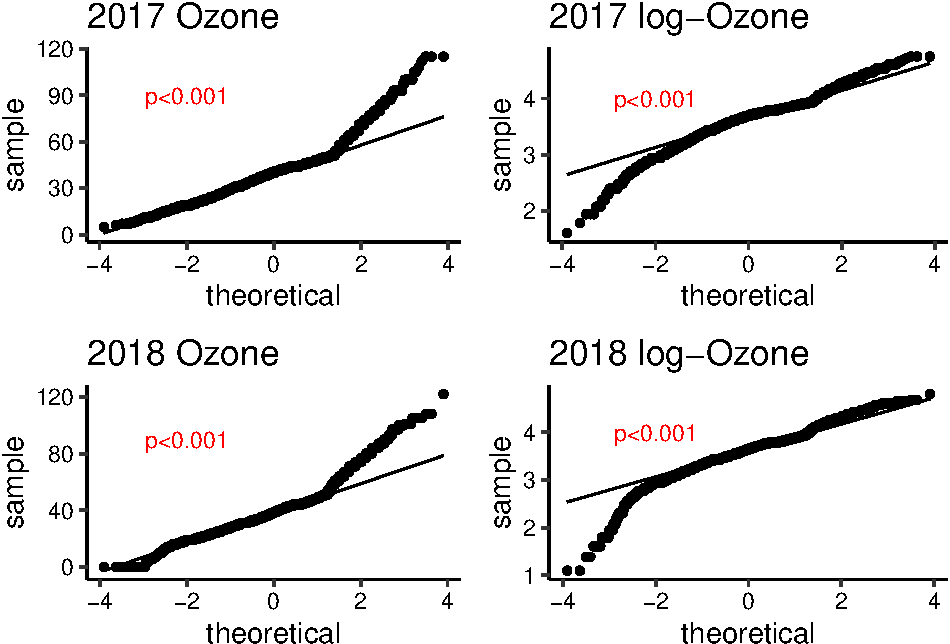
\includegraphics{Xia_ENV_872_Project_files/figure-latex/exploration 1-1.pdf}
\caption{QQ plots for 2017 and 2018 with/without log transform}
\end{figure}

\begin{figure}
\centering
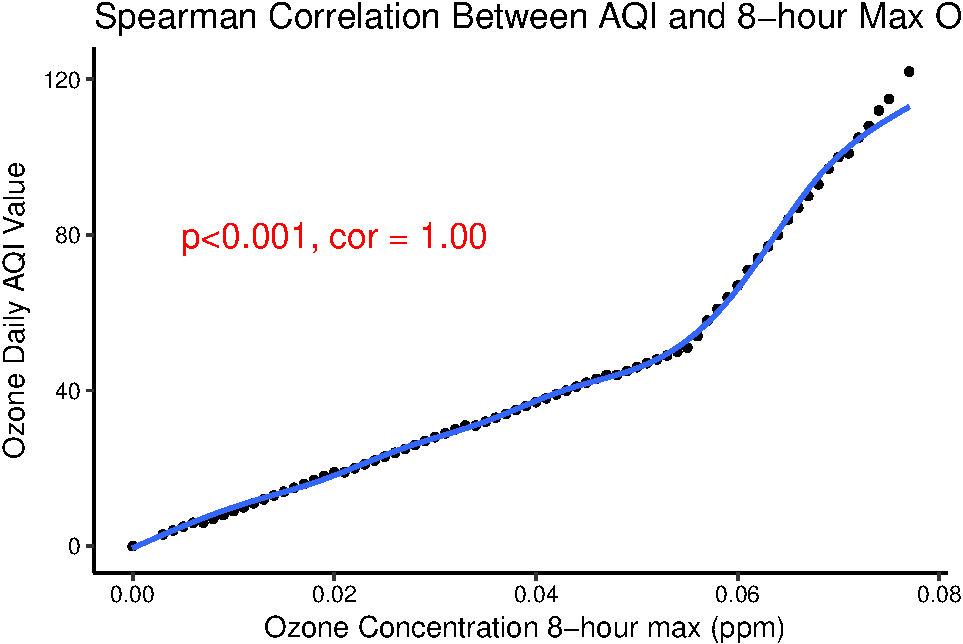
\includegraphics{Xia_ENV_872_Project_files/figure-latex/exploration 2-1.pdf}
\caption{Correlation Between AQI and 8-hour Max Ozone Concentration}
\end{figure}

\begin{figure}
\centering
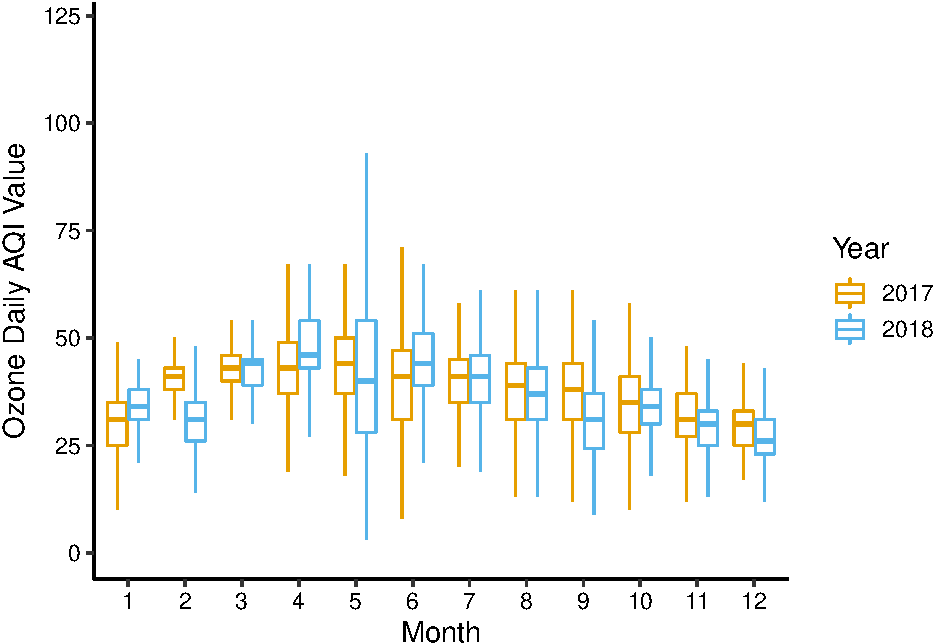
\includegraphics{Xia_ENV_872_Project_files/figure-latex/exploration 3-1.pdf}
\caption{Monthly Box Plot of 2017 and 2018 Ozone AQI}
\end{figure}

\begin{figure}
\centering
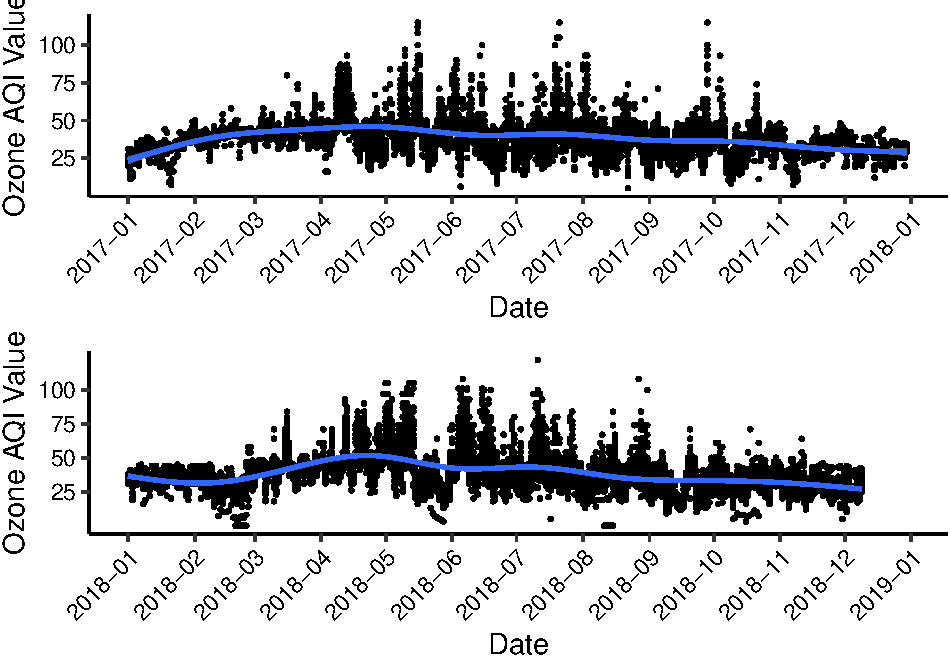
\includegraphics{Xia_ENV_872_Project_files/figure-latex/exploration 5-1.pdf}
\caption{Density Function and correlation among variables for GLM}
\end{figure}

\begin{figure}
\centering
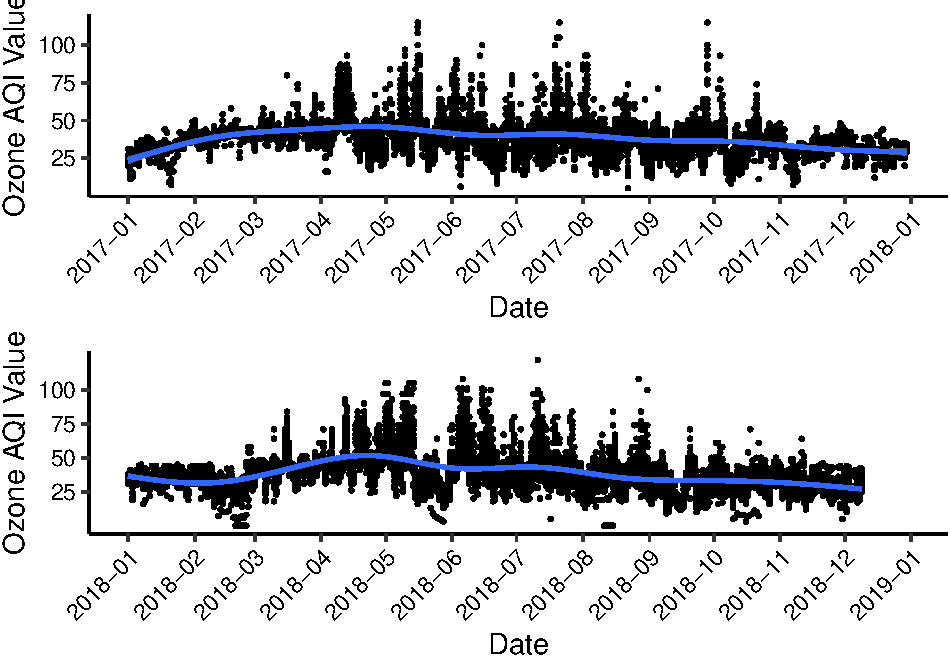
\includegraphics{Xia_ENV_872_Project_files/figure-latex/exploration 6-1.pdf}
\caption{2017 and 2018 ozone AQI change through out year}
\end{figure}

\newpage

\section{Analysis}\label{analysis}

\begin{itemize}
\item[] First analysis is the Wilcoxon test to test if ozone AQI in 2017 is lower than 2018. Wilcoxon test is conducted since the data are non-parametric data, which means not normally distributed. T-test or ANOVA test cannot be used here. Both the difference for yearly mean and monthly difference are tested. One interesting finding before conducting the test is that the 2017 AQI mean is actually higher than the 2018 AQI, so the null hypothesis is adjusted as follow:  
\item[]H0: 2017 and 2018 mean ozone AQI are identical.  \
\item[]Ha: 2017 has a higher mean ozone AQI than 2018.  \
\item[]From the result and the visualization figures we see that, the 2017 has a significantly lower mean AQI than 2018 (p-value <0.001). Among the 12 months, February (p-value <0.001), May (p-value <0.001), August (p-value <0.001), September (p-value <0.001), October (p-value = 0.04), November (p-value <0.001), December (p-value <0.001) also have higher mean ozone AQI than 2018.
\item[]While in January, April, June, the p-value is 1, and the mean of AQI in 2018 in these month are higher than 2017.
\end{itemize}

\begin{Shaded}
\begin{Highlighting}[]
\CommentTok{#ANOVA Test Assumption}
\CommentTok{#Previous tested for normality not met}
\KeywordTok{ks.test}\NormalTok{(EPA_Ozone_}\FloatTok{2017.}\NormalTok{data.Processed}\OperatorTok{$}\NormalTok{DAILY_AQI_VALUE,pnorm)}
\end{Highlighting}
\end{Shaded}

\begin{verbatim}
## Warning in ks.test(EPA_Ozone_2017.data.Processed$DAILY_AQI_VALUE, pnorm):
## ties should not be present for the Kolmogorov-Smirnov test
\end{verbatim}

\begin{verbatim}
## 
##  One-sample Kolmogorov-Smirnov test
## 
## data:  EPA_Ozone_2017.data.Processed$DAILY_AQI_VALUE
## D = 1, p-value < 2.2e-16
## alternative hypothesis: two-sided
\end{verbatim}

\begin{Shaded}
\begin{Highlighting}[]
\KeywordTok{ks.test}\NormalTok{(}\KeywordTok{log}\NormalTok{(EPA_Ozone_}\FloatTok{2017.}\NormalTok{data.Processed}\OperatorTok{$}\NormalTok{DAILY_AQI_VALUE),pnorm)}
\end{Highlighting}
\end{Shaded}

\begin{verbatim}
## Warning in ks.test(log(EPA_Ozone_2017.data.Processed$DAILY_AQI_VALUE),
## pnorm): ties should not be present for the Kolmogorov-Smirnov test
\end{verbatim}

\begin{verbatim}
## 
##  One-sample Kolmogorov-Smirnov test
## 
## data:  log(EPA_Ozone_2017.data.Processed$DAILY_AQI_VALUE)
## D = 0.99173, p-value < 2.2e-16
## alternative hypothesis: two-sided
\end{verbatim}

\begin{Shaded}
\begin{Highlighting}[]
\KeywordTok{ks.test}\NormalTok{(EPA_Ozone_}\FloatTok{2018.}\NormalTok{data.Processed}\OperatorTok{$}\NormalTok{DAILY_AQI_VALUE,pnorm)}
\end{Highlighting}
\end{Shaded}

\begin{verbatim}
## Warning in ks.test(EPA_Ozone_2018.data.Processed$DAILY_AQI_VALUE, pnorm):
## ties should not be present for the Kolmogorov-Smirnov test
\end{verbatim}

\begin{verbatim}
## 
##  One-sample Kolmogorov-Smirnov test
## 
## data:  EPA_Ozone_2018.data.Processed$DAILY_AQI_VALUE
## D = 0.99821, p-value < 2.2e-16
## alternative hypothesis: two-sided
\end{verbatim}

\begin{Shaded}
\begin{Highlighting}[]
\KeywordTok{ks.test}\NormalTok{(}\KeywordTok{log}\NormalTok{(EPA_Ozone_}\FloatTok{2018.}\NormalTok{data.Processed}\OperatorTok{$}\NormalTok{DAILY_AQI_VALUE),pnorm)}
\end{Highlighting}
\end{Shaded}

\begin{verbatim}
## Warning in ks.test(log(EPA_Ozone_2018.data.Processed$DAILY_AQI_VALUE),
## pnorm): ties should not be present for the Kolmogorov-Smirnov test
\end{verbatim}

\begin{verbatim}
## 
##  One-sample Kolmogorov-Smirnov test
## 
## data:  log(EPA_Ozone_2018.data.Processed$DAILY_AQI_VALUE)
## D = 0.98881, p-value < 2.2e-16
## alternative hypothesis: two-sided
\end{verbatim}

\begin{Shaded}
\begin{Highlighting}[]
\CommentTok{#test for homogenecity of variance met}
\KeywordTok{class}\NormalTok{(EPA_totalOzone.data.processed}\OperatorTok{$}\NormalTok{year)}
\end{Highlighting}
\end{Shaded}

\begin{verbatim}
## [1] "numeric"
\end{verbatim}

\begin{Shaded}
\begin{Highlighting}[]
\NormalTok{EPA_totalOzone.data.processed}\OperatorTok{$}\NormalTok{year <-}\StringTok{ }\KeywordTok{as.factor}\NormalTok{(EPA_totalOzone.data.processed}\OperatorTok{$}\NormalTok{year)}

\KeywordTok{sd}\NormalTok{(EPA_Ozone_}\FloatTok{2017.}\NormalTok{data.Processed}\OperatorTok{$}\NormalTok{DAILY_AQI_VALUE)}\OperatorTok{/}
\StringTok{  }\KeywordTok{sd}\NormalTok{(EPA_Ozone_}\FloatTok{2018.}\NormalTok{data.Processed}\OperatorTok{$}\NormalTok{DAILY_AQI_VALUE)}
\end{Highlighting}
\end{Shaded}

\begin{verbatim}
## [1] 0.87895
\end{verbatim}

\begin{Shaded}
\begin{Highlighting}[]
\CommentTok{# bartlett.test(EPA_totalOzone.data.processed$DAILY_AQI_VALUE~}
\CommentTok{# EPA_totalOzone.data.processed$year, EPA_totalOzone.data.processed)}
     
\CommentTok{#T-test Assumption not met, data is not normally distributed. }
\CommentTok{#So I will conduct Mann-Whitney-Wilcoxon Test.}

\KeywordTok{mean}\NormalTok{(EPA_Ozone_}\FloatTok{2017.}\NormalTok{data.Processed}\OperatorTok{$}\NormalTok{DAILY_AQI_VALUE)}
\end{Highlighting}
\end{Shaded}

\begin{verbatim}
## [1] 39.86897
\end{verbatim}

\begin{Shaded}
\begin{Highlighting}[]
\KeywordTok{mean}\NormalTok{(EPA_Ozone_}\FloatTok{2018.}\NormalTok{data.Processed}\OperatorTok{$}\NormalTok{DAILY_AQI_VALUE)}
\end{Highlighting}
\end{Shaded}

\begin{verbatim}
## [1] 39.45543
\end{verbatim}

\begin{Shaded}
\begin{Highlighting}[]
\KeywordTok{wilcox.test}\NormalTok{(EPA_Ozone_}\FloatTok{2017.}\NormalTok{data.Processed}\OperatorTok{$}\NormalTok{DAILY_AQI_VALUE,}
\NormalTok{            EPA_Ozone_}\FloatTok{2018.}\NormalTok{data.Processed}\OperatorTok{$}\NormalTok{DAILY_AQI_VALUE, }\DataTypeTok{alternative =} \StringTok{"greater"}\NormalTok{)}
\end{Highlighting}
\end{Shaded}

\begin{verbatim}
## 
##  Wilcoxon rank sum test with continuity correction
## 
## data:  EPA_Ozone_2017.data.Processed$DAILY_AQI_VALUE and EPA_Ozone_2018.data.Processed$DAILY_AQI_VALUE
## W = 58178000, p-value = 9.077e-13
## alternative hypothesis: true location shift is greater than 0
\end{verbatim}

\begin{Shaded}
\begin{Highlighting}[]
\KeywordTok{wilcox.test}\NormalTok{(month_1_}\DecValTok{2017}\OperatorTok{$}\NormalTok{DAILY_AQI_VALUE,month_1_}\DecValTok{2018}\OperatorTok{$}\NormalTok{DAILY_AQI_VALUE,}
            \DataTypeTok{alternative =} \StringTok{"greater"}\NormalTok{)}
\end{Highlighting}
\end{Shaded}

\begin{verbatim}
## 
##  Wilcoxon rank sum test with continuity correction
## 
## data:  month_1_2017$DAILY_AQI_VALUE and month_1_2018$DAILY_AQI_VALUE
## W = 30854, p-value = 1
## alternative hypothesis: true location shift is greater than 0
\end{verbatim}

\begin{Shaded}
\begin{Highlighting}[]
\KeywordTok{wilcox.test}\NormalTok{(month_2_}\DecValTok{2017}\OperatorTok{$}\NormalTok{DAILY_AQI_VALUE,month_2_}\DecValTok{2018}\OperatorTok{$}\NormalTok{DAILY_AQI_VALUE, }
            \DataTypeTok{alternative =} \StringTok{"greater"}\NormalTok{)}
\end{Highlighting}
\end{Shaded}

\begin{verbatim}
## 
##  Wilcoxon rank sum test with continuity correction
## 
## data:  month_2_2017$DAILY_AQI_VALUE and month_2_2018$DAILY_AQI_VALUE
## W = 114220, p-value < 2.2e-16
## alternative hypothesis: true location shift is greater than 0
\end{verbatim}

\begin{Shaded}
\begin{Highlighting}[]
\KeywordTok{wilcox.test}\NormalTok{(month_3_}\DecValTok{2017}\OperatorTok{$}\NormalTok{DAILY_AQI_VALUE,month_3_}\DecValTok{2018}\OperatorTok{$}\NormalTok{DAILY_AQI_VALUE, }
            \DataTypeTok{alternative =} \StringTok{"greater"}\NormalTok{)}
\end{Highlighting}
\end{Shaded}

\begin{verbatim}
## 
##  Wilcoxon rank sum test with continuity correction
## 
## data:  month_3_2017$DAILY_AQI_VALUE and month_3_2018$DAILY_AQI_VALUE
## W = 725790, p-value = 0.0865
## alternative hypothesis: true location shift is greater than 0
\end{verbatim}

\begin{Shaded}
\begin{Highlighting}[]
\KeywordTok{wilcox.test}\NormalTok{(month_4_}\DecValTok{2017}\OperatorTok{$}\NormalTok{DAILY_AQI_VALUE,month_4_}\DecValTok{2018}\OperatorTok{$}\NormalTok{DAILY_AQI_VALUE, }
            \DataTypeTok{alternative =} \StringTok{"greater"}\NormalTok{)}
\end{Highlighting}
\end{Shaded}

\begin{verbatim}
## 
##  Wilcoxon rank sum test with continuity correction
## 
## data:  month_4_2017$DAILY_AQI_VALUE and month_4_2018$DAILY_AQI_VALUE
## W = 486820, p-value = 1
## alternative hypothesis: true location shift is greater than 0
\end{verbatim}

\begin{Shaded}
\begin{Highlighting}[]
\KeywordTok{wilcox.test}\NormalTok{(month_5_}\DecValTok{2017}\OperatorTok{$}\NormalTok{DAILY_AQI_VALUE,month_5_}\DecValTok{2018}\OperatorTok{$}\NormalTok{DAILY_AQI_VALUE, }
            \DataTypeTok{alternative =} \StringTok{"greater"}\NormalTok{)}
\end{Highlighting}
\end{Shaded}

\begin{verbatim}
## 
##  Wilcoxon rank sum test with continuity correction
## 
## data:  month_5_2017$DAILY_AQI_VALUE and month_5_2018$DAILY_AQI_VALUE
## W = 794380, p-value = 1.553e-07
## alternative hypothesis: true location shift is greater than 0
\end{verbatim}

\begin{Shaded}
\begin{Highlighting}[]
\KeywordTok{wilcox.test}\NormalTok{(month_6_}\DecValTok{2017}\OperatorTok{$}\NormalTok{DAILY_AQI_VALUE,month_6_}\DecValTok{2018}\OperatorTok{$}\NormalTok{DAILY_AQI_VALUE, }
            \DataTypeTok{alternative =} \StringTok{"greater"}\NormalTok{)}
\end{Highlighting}
\end{Shaded}

\begin{verbatim}
## 
##  Wilcoxon rank sum test with continuity correction
## 
## data:  month_6_2017$DAILY_AQI_VALUE and month_6_2018$DAILY_AQI_VALUE
## W = 503450, p-value = 1
## alternative hypothesis: true location shift is greater than 0
\end{verbatim}

\begin{Shaded}
\begin{Highlighting}[]
\KeywordTok{wilcox.test}\NormalTok{(month_7_}\DecValTok{2017}\OperatorTok{$}\NormalTok{DAILY_AQI_VALUE,month_7_}\DecValTok{2018}\OperatorTok{$}\NormalTok{DAILY_AQI_VALUE, }
            \DataTypeTok{alternative =} \StringTok{"greater"}\NormalTok{)}
\end{Highlighting}
\end{Shaded}

\begin{verbatim}
## 
##  Wilcoxon rank sum test with continuity correction
## 
## data:  month_7_2017$DAILY_AQI_VALUE and month_7_2018$DAILY_AQI_VALUE
## W = 689380, p-value = 0.6059
## alternative hypothesis: true location shift is greater than 0
\end{verbatim}

\begin{Shaded}
\begin{Highlighting}[]
\KeywordTok{wilcox.test}\NormalTok{(month_8_}\DecValTok{2017}\OperatorTok{$}\NormalTok{DAILY_AQI_VALUE,month_8_}\DecValTok{2018}\OperatorTok{$}\NormalTok{DAILY_AQI_VALUE, }
            \DataTypeTok{alternative =} \StringTok{"greater"}\NormalTok{)}
\end{Highlighting}
\end{Shaded}

\begin{verbatim}
## 
##  Wilcoxon rank sum test with continuity correction
## 
## data:  month_8_2017$DAILY_AQI_VALUE and month_8_2018$DAILY_AQI_VALUE
## W = 767460, p-value = 7.514e-07
## alternative hypothesis: true location shift is greater than 0
\end{verbatim}

\begin{Shaded}
\begin{Highlighting}[]
\KeywordTok{wilcox.test}\NormalTok{(month_9_}\DecValTok{2017}\OperatorTok{$}\NormalTok{DAILY_AQI_VALUE,month_9_}\DecValTok{2018}\OperatorTok{$}\NormalTok{DAILY_AQI_VALUE, }
            \DataTypeTok{alternative =} \StringTok{"greater"}\NormalTok{)}
\end{Highlighting}
\end{Shaded}

\begin{verbatim}
## 
##  Wilcoxon rank sum test with continuity correction
## 
## data:  month_9_2017$DAILY_AQI_VALUE and month_9_2018$DAILY_AQI_VALUE
## W = 618390, p-value < 2.2e-16
## alternative hypothesis: true location shift is greater than 0
\end{verbatim}

\begin{Shaded}
\begin{Highlighting}[]
\KeywordTok{wilcox.test}\NormalTok{(month_10_}\DecValTok{2017}\OperatorTok{$}\NormalTok{DAILY_AQI_VALUE,}
\NormalTok{            month_10_}\DecValTok{2018}\OperatorTok{$}\NormalTok{DAILY_AQI_VALUE, }\DataTypeTok{alternative =} \StringTok{"greater"}\NormalTok{)}
\end{Highlighting}
\end{Shaded}

\begin{verbatim}
## 
##  Wilcoxon rank sum test with continuity correction
## 
## data:  month_10_2017$DAILY_AQI_VALUE and month_10_2018$DAILY_AQI_VALUE
## W = 607880, p-value = 0.03632
## alternative hypothesis: true location shift is greater than 0
\end{verbatim}

\begin{Shaded}
\begin{Highlighting}[]
\KeywordTok{wilcox.test}\NormalTok{(month_11_}\DecValTok{2017}\OperatorTok{$}\NormalTok{DAILY_AQI_VALUE,}
\NormalTok{            month_11_}\DecValTok{2018}\OperatorTok{$}\NormalTok{DAILY_AQI_VALUE, }\DataTypeTok{alternative =} \StringTok{"greater"}\NormalTok{)}
\end{Highlighting}
\end{Shaded}

\begin{verbatim}
## 
##  Wilcoxon rank sum test with continuity correction
## 
## data:  month_11_2017$DAILY_AQI_VALUE and month_11_2018$DAILY_AQI_VALUE
## W = 89283, p-value = 0.0003441
## alternative hypothesis: true location shift is greater than 0
\end{verbatim}

\begin{Shaded}
\begin{Highlighting}[]
\KeywordTok{wilcox.test}\NormalTok{(month_12_}\DecValTok{2017}\OperatorTok{$}\NormalTok{DAILY_AQI_VALUE,}
\NormalTok{            month_12_}\DecValTok{2018}\OperatorTok{$}\NormalTok{DAILY_AQI_VALUE, }\DataTypeTok{alternative =} \StringTok{"greater"}\NormalTok{)}
\end{Highlighting}
\end{Shaded}

\begin{verbatim}
## 
##  Wilcoxon rank sum test with continuity correction
## 
## data:  month_12_2017$DAILY_AQI_VALUE and month_12_2018$DAILY_AQI_VALUE
## W = 25216, p-value = 0.0003636
## alternative hypothesis: true location shift is greater than 0
\end{verbatim}

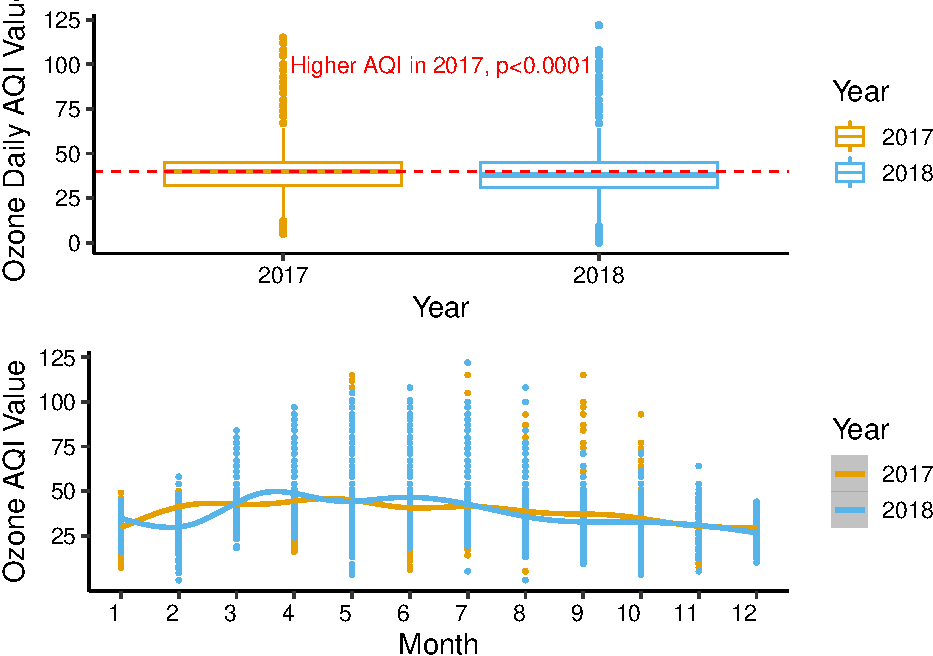
\includegraphics{Xia_ENV_872_Project_files/figure-latex/Final visualization 1-1.pdf}
\pagebreak

\begin{itemize}
\item[]The second main analysis employs the Mann-kenndal test to determine whether there is a monotonic trend combining with Pettitt's test which find the shift point in the central tendency of time series. Weather is especially favorable for ozone formation when it is hot, dry and sunny. The two tests help to understand how ozone pollution level fluctuated through a yearly time period in 2017 and 2018.
\item[]H0: There is no monotonic trend in the ozone AQI in 2017 (2018).  \
\item[]Ha: There is a trend exist.\
 In 2017, two significant change points are detected, one is on August 6th (p < 0.001), another is on October 7th (p<0.001). There is a significant positive trend from start of the year to August 6th (z = 4.65, p < 0.001), and a significant negative general trend from August 6th to the end of year (z = -4.24, p <0.001). There is also a suggestive slight positive trend from August 6th to October 7th (z = 1.80, p = 0.07), and a non-significant negative trend after October 7th (z =-1.16, p = 0.24).
\item[]In 2018, there are three significant change points are detected, on July 29th (p < 0.001), on September 9th (p<0.001), and on October 7th (p = 0.002). There is a significant positive trend from start of the year to July 29th (z = 5.66, p < 0.001), and a significant negative general trend from July 29th to the end of year (z = -3.85, p <0.001). There is also a non-significant positive trend from July 29th to September 9th (z = 1.36, p = 0.17), a significant positive trend from September 9th to October 7th (p = 0.007), a significant negative trend after October 7th (z =- 2.28, p = 0.02).
\item[]Both the result and the figure show that the trends of ozone level fluctuate are similar in 2017 and 2018. There are change points in summer/ fall in both years and the change point is on the exact same date on October 7th. And there are positive trends in first half of year (from winter to summer) and negative trends in the later part of year (from summer/fall to the following winter in end of year).
\end{itemize}

\begin{Shaded}
\begin{Highlighting}[]
\CommentTok{#Mann-Kendall test for trend of Ozone in both 2017 and 2018.}
\CommentTok{#group_by date}
\NormalTok{Ozonebydate_}\DecValTok{2017}\NormalTok{ <-}\StringTok{ }\NormalTok{EPA_Ozone_}\FloatTok{2017.}\NormalTok{data.Processed }\OperatorTok\StringTok{ }
\StringTok{   }\KeywordTok{group_by}\NormalTok{(Date) }\OperatorTok\StringTok{ }
\StringTok{  }\KeywordTok{summarise}\NormalTok{(}\DataTypeTok{MeanOzoneAQI =} \KeywordTok{mean}\NormalTok{(DAILY_AQI_VALUE))}

\NormalTok{Ozonebydate_}\DecValTok{2018}\NormalTok{ <-}\StringTok{ }\NormalTok{EPA_Ozone_}\FloatTok{2018.}\NormalTok{data.Processed }\OperatorTok\StringTok{ }
\StringTok{   }\KeywordTok{group_by}\NormalTok{(Date) }\OperatorTok\StringTok{ }
\StringTok{  }\KeywordTok{summarise}\NormalTok{(}\DataTypeTok{MeanOzoneAQI =} \KeywordTok{mean}\NormalTok{(DAILY_AQI_VALUE))}
\CommentTok{#Non-normal data 2017:}

\CommentTok{#Test for Change point}
\KeywordTok{pettitt.test}\NormalTok{(Ozonebydate_}\DecValTok{2017}\OperatorTok{$}\NormalTok{MeanOzoneAQI)}
\end{Highlighting}
\end{Shaded}

\begin{verbatim}
## 
##  Pettitt's test for single change-point detection
## 
## data:  Ozonebydate_2017$MeanOzoneAQI
## U* = 14903, p-value = 2.158e-12
## alternative hypothesis: two.sided
## sample estimates:
## probable change point at time K 
##                             218
\end{verbatim}

\begin{Shaded}
\begin{Highlighting}[]
\CommentTok{# 218: 2017-08-06}

\CommentTok{# Run seperate Mann-Kendall for each change point: possitive trend}
  \KeywordTok{mk.test}\NormalTok{(Ozonebydate_}\DecValTok{2017}\OperatorTok{$}\NormalTok{MeanOzoneAQI[}\DecValTok{1}\OperatorTok{:}\DecValTok{218}\NormalTok{])}
\end{Highlighting}
\end{Shaded}

\begin{verbatim}
## 
##  Mann-Kendall trend test
## 
## data:  Ozonebydate_2017$MeanOzoneAQI[1:218]
## z = 4.6491, n = 218, p-value = 3.334e-06
## alternative hypothesis: true S is not equal to 0
## sample estimates:
##            S         varS          tau 
## 5.006000e+03 1.158979e+06 2.117105e-01
\end{verbatim}

\begin{Shaded}
\begin{Highlighting}[]
  \CommentTok{#negative trend}
\KeywordTok{mk.test}\NormalTok{(Ozonebydate_}\DecValTok{2017}\OperatorTok{$}\NormalTok{MeanOzoneAQI[}\DecValTok{218}\OperatorTok{:}\DecValTok{364}\NormalTok{])}
\end{Highlighting}
\end{Shaded}

\begin{verbatim}
## 
##  Mann-Kendall trend test
## 
## data:  Ozonebydate_2017$MeanOzoneAQI[218:364]
## z = -4.2373, n = 147, p-value = 2.262e-05
## alternative hypothesis: true S is not equal to 0
## sample estimates:
##             S          varS           tau 
## -2.531000e+03  3.564963e+05 -2.359687e-01
\end{verbatim}

\begin{Shaded}
\begin{Highlighting}[]
\CommentTok{#Another Change point at 280 : 2017-10-07}
\KeywordTok{pettitt.test}\NormalTok{(Ozonebydate_}\DecValTok{2017}\OperatorTok{$}\NormalTok{MeanOzoneAQI[}\DecValTok{218}\OperatorTok{:}\DecValTok{364}\NormalTok{]) }
\end{Highlighting}
\end{Shaded}

\begin{verbatim}
## 
##  Pettitt's test for single change-point detection
## 
## data:  Ozonebydate_2017$MeanOzoneAQI[218:364]
## U* = 2666, p-value = 3.236e-06
## alternative hypothesis: two.sided
## sample estimates:
## probable change point at time K 
##                              62
\end{verbatim}

\begin{Shaded}
\begin{Highlighting}[]
\KeywordTok{mk.test}\NormalTok{(Ozonebydate_}\DecValTok{2017}\OperatorTok{$}\NormalTok{MeanOzoneAQI[}\DecValTok{218}\OperatorTok{:}\DecValTok{280}\NormalTok{]) }\CommentTok{#no significant trend}
\end{Highlighting}
\end{Shaded}

\begin{verbatim}
## 
##  Mann-Kendall trend test
## 
## data:  Ozonebydate_2017$MeanOzoneAQI[218:280]
## z = 1.8031, n = 63, p-value = 0.07138
## alternative hypothesis: true S is not equal to 0
## sample estimates:
##          S       varS        tau 
## 3.0500e+02 2.8427e+04 1.5617e-01
\end{verbatim}

\begin{Shaded}
\begin{Highlighting}[]
\KeywordTok{mk.test}\NormalTok{(Ozonebydate_}\DecValTok{2017}\OperatorTok{$}\NormalTok{MeanOzoneAQI[}\DecValTok{281}\OperatorTok{:}\DecValTok{364}\NormalTok{]) }\CommentTok{#no significant trend}
\end{Highlighting}
\end{Shaded}

\begin{verbatim}
## 
##  Mann-Kendall trend test
## 
## data:  Ozonebydate_2017$MeanOzoneAQI[281:364]
## z = -1.1551, n = 84, p-value = 0.248
## alternative hypothesis: true S is not equal to 0
## sample estimates:
##             S          varS           tau 
## -3.000000e+02  6.699933e+04 -8.615744e-02
\end{verbatim}

\begin{Shaded}
\begin{Highlighting}[]
\CommentTok{#anythird change point?}
\KeywordTok{pettitt.test}\NormalTok{(Ozonebydate_}\DecValTok{2017}\OperatorTok{$}\NormalTok{MeanOzoneAQI[}\DecValTok{281}\OperatorTok{:}\DecValTok{364}\NormalTok{]) }\CommentTok{#not significant}
\end{Highlighting}
\end{Shaded}

\begin{verbatim}
## 
##  Pettitt's test for single change-point detection
## 
## data:  Ozonebydate_2017$MeanOzoneAQI[281:364]
## U* = 566, p-value = 0.08113
## alternative hypothesis: two.sided
## sample estimates:
## probable change point at time K 
##                              59
\end{verbatim}

\begin{Shaded}
\begin{Highlighting}[]
\CommentTok{#Non-normal data 2018:}

\CommentTok{#Test for Change point}
\KeywordTok{pettitt.test}\NormalTok{(Ozonebydate_}\DecValTok{2018}\OperatorTok{$}\NormalTok{MeanOzoneAQI)}
\end{Highlighting}
\end{Shaded}

\begin{verbatim}
## 
##  Pettitt's test for single change-point detection
## 
## data:  Ozonebydate_2018$MeanOzoneAQI
## U* = 14869, p-value = 1.165e-14
## alternative hypothesis: two.sided
## sample estimates:
## probable change point at time K 
##                             210
\end{verbatim}

\begin{Shaded}
\begin{Highlighting}[]
\CommentTok{# 210: 2018-07-29}

\CommentTok{# Run seperate Mann-Kendall for each change point: possitive trend}
  \KeywordTok{mk.test}\NormalTok{(Ozonebydate_}\DecValTok{2018}\OperatorTok{$}\NormalTok{MeanOzoneAQI[}\DecValTok{1}\OperatorTok{:}\DecValTok{210}\NormalTok{])}
\end{Highlighting}
\end{Shaded}

\begin{verbatim}
## 
##  Mann-Kendall trend test
## 
## data:  Ozonebydate_2018$MeanOzoneAQI[1:210]
## z = 5.6612, n = 210, p-value = 1.503e-08
## alternative hypothesis: true S is not equal to 0
## sample estimates:
##            S         varS          tau 
## 5.764000e+03 1.036289e+06 2.626746e-01
\end{verbatim}

\begin{Shaded}
\begin{Highlighting}[]
  \CommentTok{#negative trend}
\KeywordTok{mk.test}\NormalTok{(Ozonebydate_}\DecValTok{2018}\OperatorTok{$}\NormalTok{MeanOzoneAQI[}\DecValTok{210}\OperatorTok{:}\DecValTok{343}\NormalTok{])}
\end{Highlighting}
\end{Shaded}

\begin{verbatim}
## 
##  Mann-Kendall trend test
## 
## data:  Ozonebydate_2018$MeanOzoneAQI[210:343]
## z = -3.8546, n = 134, p-value = 0.0001159
## alternative hypothesis: true S is not equal to 0
## sample estimates:
##             S          varS           tau 
## -2.005000e+03  2.702983e+05 -2.250281e-01
\end{verbatim}

\begin{Shaded}
\begin{Highlighting}[]
\CommentTok{#Another Change point at 252 : 2017-09-09}
\KeywordTok{pettitt.test}\NormalTok{(Ozonebydate_}\DecValTok{2018}\OperatorTok{$}\NormalTok{MeanOzoneAQI[}\DecValTok{210}\OperatorTok{:}\DecValTok{343}\NormalTok{]) }
\end{Highlighting}
\end{Shaded}

\begin{verbatim}
## 
##  Pettitt's test for single change-point detection
## 
## data:  Ozonebydate_2018$MeanOzoneAQI[210:343]
## U* = 1957, p-value = 0.0001528
## alternative hypothesis: two.sided
## sample estimates:
## probable change point at time K 
##                              42
\end{verbatim}

\begin{Shaded}
\begin{Highlighting}[]
\KeywordTok{mk.test}\NormalTok{(Ozonebydate_}\DecValTok{2018}\OperatorTok{$}\NormalTok{MeanOzoneAQI[}\DecValTok{210}\OperatorTok{:}\DecValTok{252}\NormalTok{]) }\CommentTok{#no significant trend}
\end{Highlighting}
\end{Shaded}

\begin{verbatim}
## 
##  Mann-Kendall trend test
## 
## data:  Ozonebydate_2018$MeanOzoneAQI[210:252]
## z = 1.3605, n = 43, p-value = 0.1737
## alternative hypothesis: true S is not equal to 0
## sample estimates:
##           S        varS         tau 
##  131.000000 9130.333333    0.145072
\end{verbatim}

\begin{Shaded}
\begin{Highlighting}[]
\KeywordTok{mk.test}\NormalTok{(Ozonebydate_}\DecValTok{2018}\OperatorTok{$}\NormalTok{MeanOzoneAQI[}\DecValTok{252}\OperatorTok{:}\DecValTok{343}\NormalTok{]) }\CommentTok{#no significant trend}
\end{Highlighting}
\end{Shaded}

\begin{verbatim}
## 
##  Mann-Kendall trend test
## 
## data:  Ozonebydate_2018$MeanOzoneAQI[252:343]
## z = -0.74202, n = 92, p-value = 0.4581
## alternative hypothesis: true S is not equal to 0
## sample estimates:
##             S          varS           tau 
## -2.210000e+02  8.790500e+04 -5.280134e-02
\end{verbatim}

\begin{Shaded}
\begin{Highlighting}[]
\CommentTok{#anythird change point? }
\KeywordTok{pettitt.test}\NormalTok{(Ozonebydate_}\DecValTok{2017}\OperatorTok{$}\NormalTok{MeanOzoneAQI[}\DecValTok{252}\OperatorTok{:}\DecValTok{343}\NormalTok{]) }\CommentTok{#At 280, 2018-10-07}
\end{Highlighting}
\end{Shaded}

\begin{verbatim}
## 
##  Pettitt's test for single change-point detection
## 
## data:  Ozonebydate_2017$MeanOzoneAQI[252:343]
## U* = 938, p-value = 0.002446
## alternative hypothesis: two.sided
## sample estimates:
## probable change point at time K 
##                              28
\end{verbatim}

\begin{Shaded}
\begin{Highlighting}[]
\KeywordTok{mk.test}\NormalTok{(Ozonebydate_}\DecValTok{2018}\OperatorTok{$}\NormalTok{MeanOzoneAQI[}\DecValTok{252}\OperatorTok{:}\DecValTok{280}\NormalTok{])}
\end{Highlighting}
\end{Shaded}

\begin{verbatim}
## 
##  Mann-Kendall trend test
## 
## data:  Ozonebydate_2018$MeanOzoneAQI[252:280]
## z = 2.6824, n = 29, p-value = 0.00731
## alternative hypothesis: true S is not equal to 0
## sample estimates:
##            S         varS          tau 
##  144.0000000 2842.0000000    0.3546798
\end{verbatim}

\begin{Shaded}
\begin{Highlighting}[]
\KeywordTok{mk.test}\NormalTok{(Ozonebydate_}\DecValTok{2018}\OperatorTok{$}\NormalTok{MeanOzoneAQI[}\DecValTok{280}\OperatorTok{:}\DecValTok{343}\NormalTok{])}
\end{Highlighting}
\end{Shaded}

\begin{verbatim}
## 
##  Mann-Kendall trend test
## 
## data:  Ozonebydate_2018$MeanOzoneAQI[280:343]
## z = -2.2827, n = 64, p-value = 0.02245
## alternative hypothesis: true S is not equal to 0
## sample estimates:
##             S          varS           tau 
##  -395.0000000 29791.0000000    -0.1959812
\end{verbatim}

\pagebreak

\begin{figure}
\centering
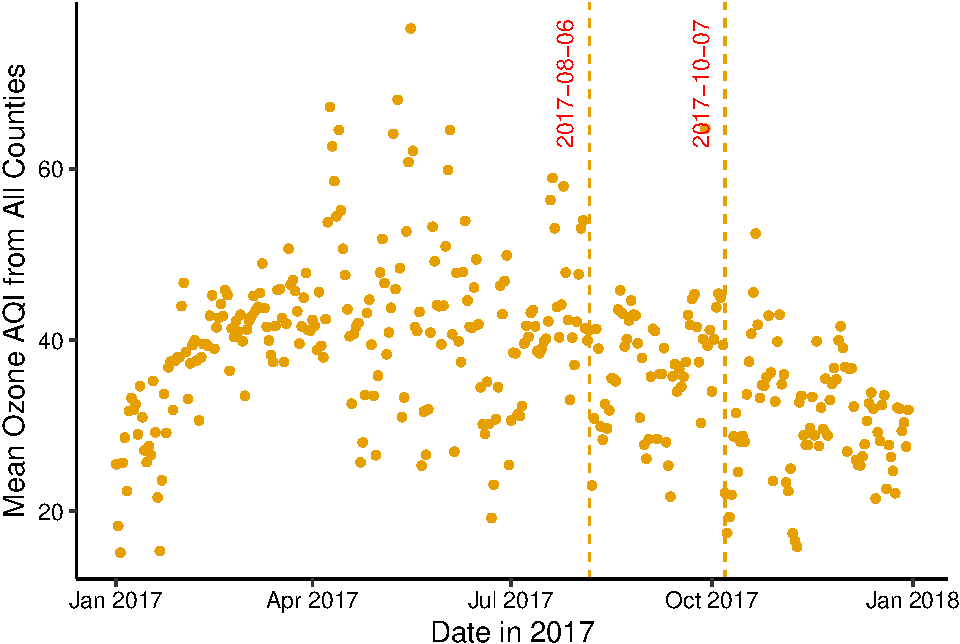
\includegraphics{Xia_ENV_872_Project_files/figure-latex/Final visualization 2-1.pdf}
\caption{2017 ozone trend}
\end{figure}

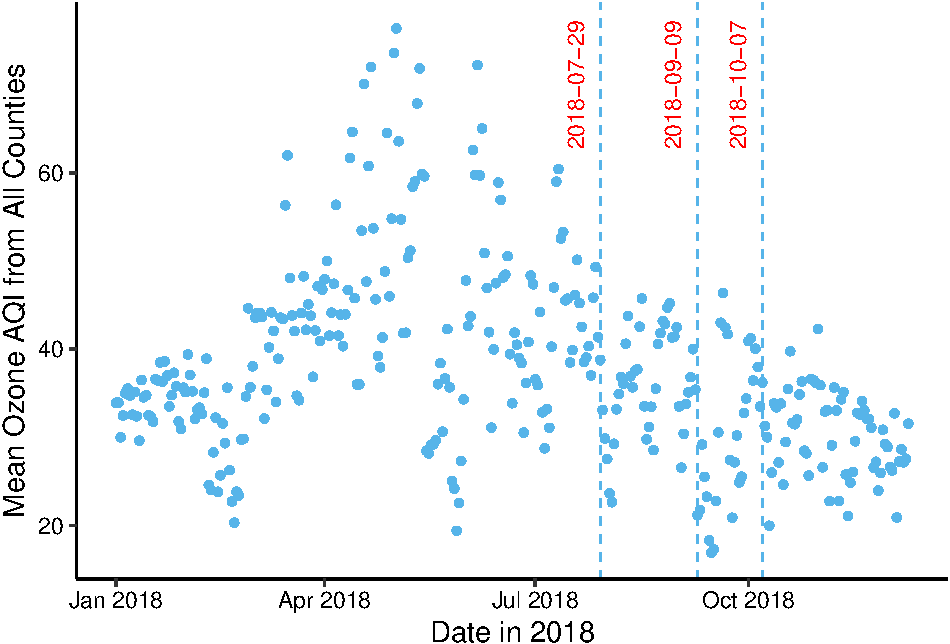
\includegraphics{Xia_ENV_872_Project_files/figure-latex/Final visualization 3-1.pdf}
\pagebreak

\begin{itemize}
\item[]The third analysis is the generalized linear model to test whether population, density, or income is correlated with Ozone AQI level. Random effect for county is included in the model.
\item[]H0: There is no significant correlation for all the variables, all the coefficients are zero. 
\item[]Ha: At least one variable is significant.
\item[]After testing the data, I found out that only the mean AQI value (p-value = 0.73) passed the Shapiro-Wilk normality test. Other variables are not normally distributed. The initial model established included all the variables, and then based on the AIC score, best fit model is selected which is MeanOzoneAQI  ~ Population (P = 0.07). Due to a small sample size, a p value of 0.07 is considered to be suggestive significant. The diagnostic residual plot shows that the residuals are evenly distributed above and below the center, so there is no skew problem.
\item[]From the result, our final model is: Mean Ozone AQI = 38.35 + 0.08 x Population. The intercept is 38.35, which means that when population is 0, there will be a mean AQI Ozone value of 38.35. And every single person increase in population will result in a 0.08 increase in the mean Ozone AQI.
\end{itemize}

\begin{Shaded}
\begin{Highlighting}[]
\CommentTok{#Generalized linear model.}
\NormalTok{LG <-}\StringTok{ }\KeywordTok{read.csv}\NormalTok{(}\StringTok{"../Processed data/OzoneSummary1.csv"}\NormalTok{)}
\KeywordTok{library}\NormalTok{(lme4)}
\end{Highlighting}
\end{Shaded}

\begin{verbatim}
## Loading required package: Matrix
\end{verbatim}

\begin{verbatim}
## 
## Attaching package: 'Matrix'
\end{verbatim}

\begin{verbatim}
## The following object is masked from 'package:tidyr':
## 
##     expand
\end{verbatim}

\begin{Shaded}
\begin{Highlighting}[]
\CommentTok{#Density =(population/square mile)}
\CommentTok{#normaility -test : not normal}
\KeywordTok{shapiro.test}\NormalTok{(FLG}\OperatorTok{$}\NormalTok{Population)}
\end{Highlighting}
\end{Shaded}

\begin{verbatim}
## 
##  Shapiro-Wilk normality test
## 
## data:  FLG$Population
## W = 0.95153, p-value = 0.01467
\end{verbatim}

\begin{Shaded}
\begin{Highlighting}[]
\KeywordTok{shapiro.test}\NormalTok{(FLG}\OperatorTok{$}\NormalTok{Income)}
\end{Highlighting}
\end{Shaded}

\begin{verbatim}
## 
##  Shapiro-Wilk normality test
## 
## data:  FLG$Income
## W = 0.90107, p-value = 9.929e-05
\end{verbatim}

\begin{Shaded}
\begin{Highlighting}[]
\KeywordTok{shapiro.test}\NormalTok{(FLG}\OperatorTok{$}\NormalTok{Density)}
\end{Highlighting}
\end{Shaded}

\begin{verbatim}
## 
##  Shapiro-Wilk normality test
## 
## data:  FLG$Density
## W = 0.71204, p-value = 8.183e-10
\end{verbatim}

\begin{Shaded}
\begin{Highlighting}[]
\CommentTok{#Normal}
\KeywordTok{shapiro.test}\NormalTok{(FLG}\OperatorTok{$}\NormalTok{MeanOzoneAQI)}
\end{Highlighting}
\end{Shaded}

\begin{verbatim}
## 
##  Shapiro-Wilk normality test
## 
## data:  FLG$MeanOzoneAQI
## W = 0.98676, p-value = 0.7344
\end{verbatim}

\begin{Shaded}
\begin{Highlighting}[]
\CommentTok{#Counties as a mixed effect}
\NormalTok{MLG <-}\StringTok{ }\NormalTok{LG }\OperatorTok\StringTok{ }
\StringTok{  }\KeywordTok{select}\NormalTok{(MeanOzoneAQI, Population, Income, Density,COUNTY) }
\NormalTok{MLG}\OperatorTok{$}\NormalTok{Population <-}\StringTok{  }\KeywordTok{as.numeric}\NormalTok{(FLG}\OperatorTok{$}\NormalTok{Population)}
\NormalTok{MLG}\OperatorTok{$}\NormalTok{Income <-}\StringTok{  }\KeywordTok{as.numeric}\NormalTok{(FLG}\OperatorTok{$}\NormalTok{Income)}
\NormalTok{MLG}\OperatorTok{$}\NormalTok{Density <-}\StringTok{  }\KeywordTok{as.numeric}\NormalTok{(FLG}\OperatorTok{$}\NormalTok{Density)}

\NormalTok{glm1 <-}\StringTok{ }\KeywordTok{lmer}\NormalTok{(}\DataTypeTok{data =}\NormalTok{ MLG, MeanOzoneAQI }\OperatorTok{~}\NormalTok{Population }\OperatorTok{+}\StringTok{ }\NormalTok{Income }\OperatorTok{+}\StringTok{ }\NormalTok{Density}\OperatorTok{+}\NormalTok{(}\DecValTok{1}\OperatorTok{|}\NormalTok{COUNTY) )}
\end{Highlighting}
\end{Shaded}

\begin{verbatim}
## Warning: Some predictor variables are on very different scales: consider
## rescaling
\end{verbatim}

\begin{Shaded}
\begin{Highlighting}[]
\NormalTok{glm2 <-}\KeywordTok{lmer}\NormalTok{(}\DataTypeTok{data =}\NormalTok{ MLG, MeanOzoneAQI }\OperatorTok{~}\NormalTok{Population }\OperatorTok{+}\StringTok{ }\NormalTok{(}\DecValTok{1}\OperatorTok{|}\NormalTok{COUNTY))}
\KeywordTok{summary}\NormalTok{(glm1)}
\end{Highlighting}
\end{Shaded}

\begin{verbatim}
## Linear mixed model fit by REML ['lmerMod']
## Formula: MeanOzoneAQI ~ Population + Income + Density + (1 | COUNTY)
##    Data: MLG
## 
## REML criterion at convergence: 298
## 
## Scaled residuals: 
##      Min       1Q   Median       3Q      Max 
## -1.54194 -0.57372  0.07852  0.56102  1.59841 
## 
## Random effects:
##  Groups   Name        Variance Std.Dev.
##  COUNTY   (Intercept) 6.483    2.546   
##  Residual             1.223    1.106   
## Number of obs: 63, groups:  COUNTY, 32
## 
## Fixed effects:
##              Estimate Std. Error t value
## (Intercept) 3.639e+01  2.955e+00  12.314
## Population  9.986e-02  5.431e-02   1.839
## Income      2.487e-05  6.501e-05   0.382
## Density     1.251e-03  1.609e-03   0.778
## 
## Correlation of Fixed Effects:
##            (Intr) Popltn Income
## Population -0.366              
## Income     -0.913  0.016       
## Density     0.374  0.259 -0.620
## fit warnings:
## Some predictor variables are on very different scales: consider rescaling
\end{verbatim}

\begin{Shaded}
\begin{Highlighting}[]
\KeywordTok{AIC}\NormalTok{(glm1)}
\end{Highlighting}
\end{Shaded}

\begin{verbatim}
## [1] 310.0305
\end{verbatim}

\begin{Shaded}
\begin{Highlighting}[]
\KeywordTok{summary}\NormalTok{(glm2)}
\end{Highlighting}
\end{Shaded}

\begin{verbatim}
## Linear mixed model fit by REML ['lmerMod']
## Formula: MeanOzoneAQI ~ Population + (1 | COUNTY)
##    Data: MLG
## 
## REML criterion at convergence: 270.9
## 
## Scaled residuals: 
##      Min       1Q   Median       3Q      Max 
## -1.53118 -0.64085  0.06108  0.52879  1.53735 
## 
## Random effects:
##  Groups   Name        Variance Std.Dev.
##  COUNTY   (Intercept) 6.447    2.539   
##  Residual             1.222    1.105   
## Number of obs: 63, groups:  COUNTY, 32
## 
## Fixed effects:
##             Estimate Std. Error t value
## (Intercept) 38.35664    0.96173  39.883
## Population   0.07543    0.05088   1.483
## 
## Correlation of Fixed Effects:
##            (Intr)
## Population -0.872
\end{verbatim}

\begin{Shaded}
\begin{Highlighting}[]
\KeywordTok{AIC}\NormalTok{(glm2)}
\end{Highlighting}
\end{Shaded}

\begin{verbatim}
## [1] 278.8938
\end{verbatim}

\begin{figure}
\centering
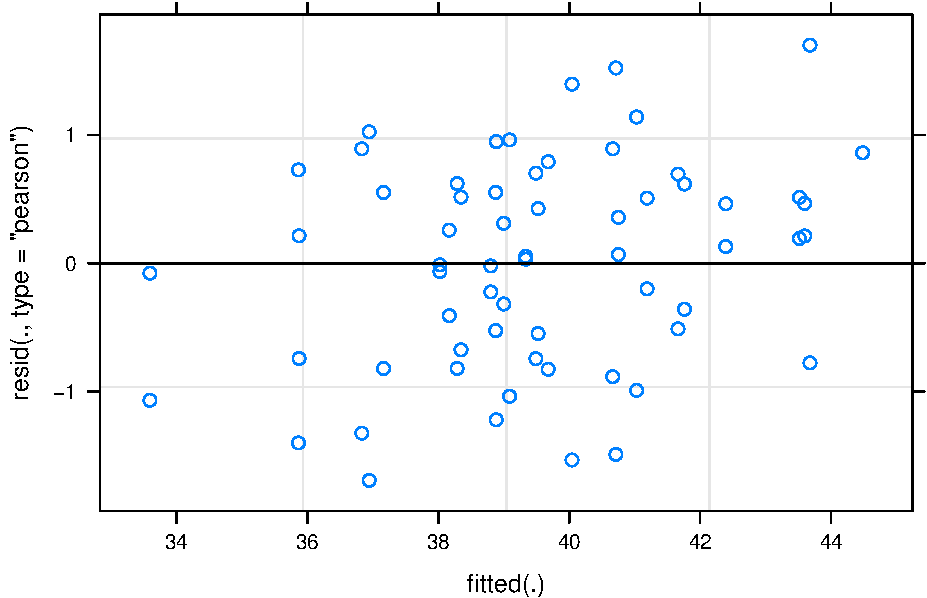
\includegraphics{Xia_ENV_872_Project_files/figure-latex/Final visualization 5-1.pdf}
\caption{Residual Plot}
\end{figure}

\begin{figure}
\centering
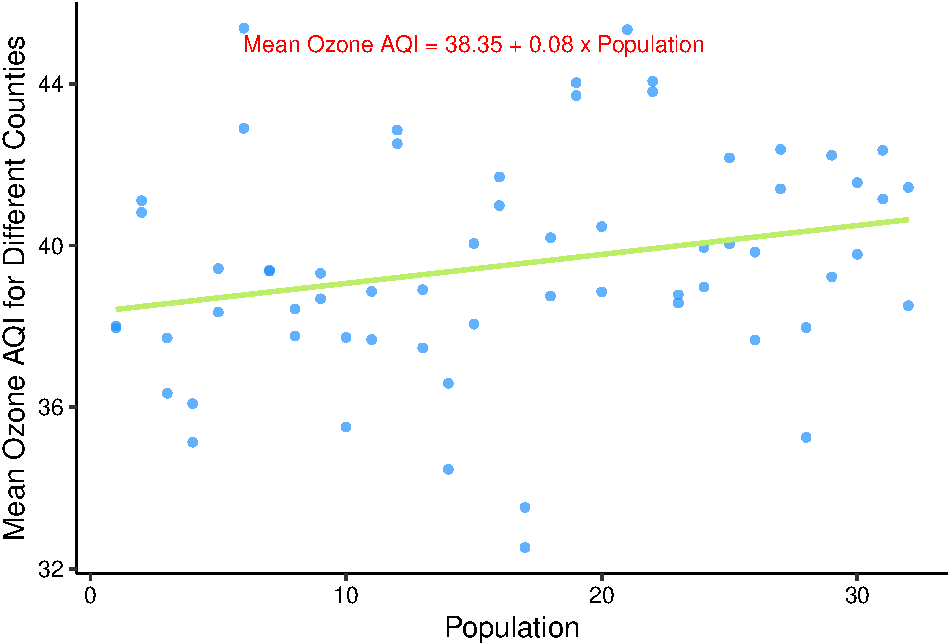
\includegraphics{Xia_ENV_872_Project_files/figure-latex/Final visualization 4-1.pdf}
\caption{Relationship Between Ozone AQI and Population}
\end{figure}

\newpage

\section{Summary and Conclusions}\label{summary-and-conclusions}


\end{document}
